\documentclass[../main.tex]{subfiles}
\begin{document}
    \chapter{Research}\label{ch:research}

    The research is executed in 3 main steps.
    The first step creates an $M^3$ model for a PHP program which contains various facts about the program. 
    The creation of an $M^3$ for PHP is explained in more details in section \ref{sec:m3_for_php}.
    Once the $M^3$ model is constructed, the second step is to extract constraints from the program using the $M^3$ model. How and which constraints are extracted is described in section \ref{sec:constraint_extraction}.
    In the third step, in section \ref{sec:research:constraint_solving}, the constraints are solved and resolve the types of variables used in the program.
    The final section \ref{sec:annotations} of this chapter explains how annotations can be included in the process to gain more precise results.
    
    \section{$M^3$ for PHP}\label{sec:m3_for_php}
    As explained in section \ref{sec:background_rascal}, $M^3$ is a language independent meta model which holds facts about programs.
    The model can be extended with language specific elements and will be used to query the system for facts about the system.
    An overview how an $M^3$ for PHP is build is shown in figure \ref{fig:research_m3_creation}.
    Independent $M^3$ models are build each PHP file in the program.
    
    \begin{figure}[H]
        \centerline{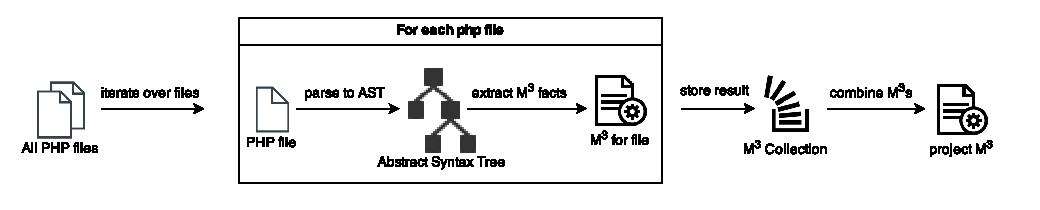
\includegraphics{Diagrams/M3Creation.pdf}}
        \caption{$M^3$ Creation}
        \label{fig:research_m3_creation}
    \end{figure}
    
    All these individual $M^3$'s are in the end combined to collect all the facts about a program.
    This results in one $M^3$ for the whole program.
    $M^3$'s are first created for each file is because it is not defined what the dependencies of a individual file are.
    There is no main file, and all files can load each other.
    In this research we assume that all files in a program are loaded when needed using autoloaders or manual includes.
    
    \subsection{Core elements}
    The $M^3$ model has the following core elements: \texttt{declarations}, \texttt{containment}, \texttt{modifiers}, \texttt{uses}, \texttt{names}, and \texttt{documentation}.
    The rascal code is displayed in Rascal \ref{fig:m3_core_elements}. The characteristics of the elements are described in the paragraphs below.

    \begin{program}    
    \begin{rascal}%%%%%%%%%%%%%%%%%%{ RASCAL }%%%%%%%%%%%%%%%%%%
\CAT{Keyword}{anno} \CAT{Keyword}{rel}{}[\CAT{Keyword}{loc} name, \CAT{Keyword}{loc} src] M3@declarations; \CAT{Comment}{// maps declarations to file location.}
\CAT{Keyword}{anno} \CAT{Keyword}{rel}{}[\CAT{Keyword}{loc} from, \CAT{Keyword}{loc} to] M3@containment; \CAT{Comment}{// what is logically contained in what else}
\CAT{Keyword}{anno} \CAT{Keyword}{rel}{}[\CAT{Keyword}{loc} definition, Modifier modifier] M3@modifiers; \CAT{Comment}{// associated modifiers}
\CAT{Keyword}{anno} \CAT{Keyword}{rel}{}[\CAT{Keyword}{loc} src, \CAT{Keyword}{loc} name] M3@uses; \CAT{Comment}{// maps src locations of usages to the declarations}
\CAT{Keyword}{anno} \CAT{Keyword}{rel}{}[\CAT{Keyword}{str} simpleName, \CAT{Keyword}{loc} qualifiedName] M3@names; \CAT{Comment}{// end-user readable names}
\CAT{Keyword}{anno} \CAT{Keyword}{rel}{}[\CAT{Keyword}{loc} definition, \CAT{Keyword}{loc} comments] M3@documentation; \CAT{Comment}{// comments and doc-blocks}\end{rascal}%%%%%%%%%%%%%%%%%%{ RASCAL }%%%%%%%%%%%%%%%%%%
	
	\caption{$M^3$ core definitions in Rascal}
	\label{fig:m3_core_elements}
	\end{program}
	    
    \paragraph{Declarations} \texttt{Declarations} defines the declarations of namespaces, classes, interfaces, traits, methods, functions, and variables and holds the relation between the logical name (which is used to refer to the declaration) and the actual file location (which is the physical place in the file system.
    For example the logical name of a class can be \texttt{$\vert$php+class://SomeNameSpace/ClassX$\vert$} while the actual location might be \texttt{$\vert$file:///project/SomeNameSpace/ClassX.php$\vert$}.
    
    \paragraph{Containment} \texttt{Containment} holds information about what elements logically contain other elements.
    For example, a property or method is contained in a class and a class is contained in a package.
    When a function is declared in another function, they are both logically contained in the global namespace (the highest level) because all functions are declared as first class citizens in PHP.
    
    \paragraph{Modifiers} \texttt{Modifiers} element contains information about the modifiers of classes, fields, and methods. 
    Classes can only be \texttt{abstract}, fields can be \texttt{public}, \texttt{private}, or \texttt{protected}, and methods can be all of them. 
    Abstract methods can only be declared in abstract classes. 
    Classes are implicitly public.
    
    \paragraph{Uses} \texttt{Uses} relation holds information about the usages of certain elements.
    It is the relation between the usage and the declaration.
    For example when you instantiate a class, in that case you 'use' that specific class.
     
    \paragraph{Names} \texttt{Names} contains the declaration and a simplified version of the name.
    The declared name can be long and unreadable.
    \texttt{names} contains human readable name which can be used for presenting the element in a GUI.
    
    \paragraph{Documentation} \texttt{Documentation} contains the link to the documentation related to the source code element.
    The link is mapped to a declaration.
    
    \subsection{PHP specific elements}
    Because every programming language differs in syntax and semantics, the $M^3$ model is extensible to provide language specific elements.
    The following php specific items are added: \texttt{extends}, \texttt{implements}, \texttt{traitUses}, \texttt{parameters}, \texttt{constructors}, \texttt{aliases}, and \texttt{annotations}.
    These PHP specific elements are described in more detail in the paragraphs below.

    \begin{program}    
    \begin{rascal}%%%%%%%%%%%%%%%%%%{ RASCAL }%%%%%%%%%%%%%%%%%%
\CAT{Keyword}{anno} \CAT{Keyword}{rel}{}[\CAT{Keyword}{loc} from, \CAT{Keyword}{loc} to] M3@extends;    \CAT{Comment}{// which class extends which class}
\CAT{Keyword}{anno} \CAT{Keyword}{rel}{}[\CAT{Keyword}{loc} from, \CAT{Keyword}{loc} to] M3@implements; \CAT{Comment}{// interface usages}
\CAT{Keyword}{anno} \CAT{Keyword}{rel}{}[\CAT{Keyword}{loc} from, \CAT{Keyword}{loc} to] M3@traitUses;  \CAT{Comment}{// trait usages}
\CAT{Keyword}{anno} \CAT{Keyword}{rel}{}[\CAT{Keyword}{loc} decl, PhpParams params] M3@parameters; \CAT{Comment}{// formal functions/methods parameters}
\CAT{Keyword}{anno} \CAT{Keyword}{rel}{}[\CAT{Keyword}{loc} decl, \CAT{Keyword}{loc} to] M3@constructors; \CAT{Comment}{// constructor usages}
\CAT{Keyword}{anno} \CAT{Keyword}{rel}{}[\CAT{Keyword}{loc} from, \CAT{Keyword}{loc} to] M3@aliases;      \CAT{Comment}{// class name aliases (new name -\textgreater{} old name)}
\CAT{Keyword}{anno} \CAT{Keyword}{rel}{}[\CAT{Keyword}{loc} pos, Annotation annotation] M3@annotations; \CAT{Comment}{// annotations from doc blocks}\end{rascal}%%%%%%%%%%%%%%%%%%{ RASCAL }%%%%%%%%%%%%%%%%%%
	
	\caption{PHP specific $M^3$ element}
	\label{fig:m3_php_elements}
	\end{program}
	    
	\paragraph{Extends} \texttt{Extends} contains information about what classes and interface extend other classes or interfaces.
	Please note that we do not hold information about which class implements which interface, because that information is contained in the \texttt{implements} relation.
    Interface extensions work just like class extensions.
    
    \paragraph{Implements} \texttt{Implements} holds information on which class implements which interfaces.
    One class can implement no, one, or multiple interfaces.
    Because the information is a relation between the class and the interface, we can easily add multiple interfaces to one class in the model.
    
    \paragraph{TraitUses} \texttt{TraitUses} lists which traits are used by which class or trait.
    A traits is a collection of reusable functions, defined in the namespace scope.
    One class can have multiple trait usages.
    All the methods of a trait are on runtime imported in the class.
    
    \paragraph{Parameters} \texttt{Parameters} keeps track of the parameters of a method or function.
    \texttt{PhpParams} is a list relation and contains the optional typehint, if the parameter is required and if it is passed as reference.
    This information is stored to make it easier to resolve the call to a method or function.
    
    \paragraph{Constructors} \texttt{Constructors} lists the constructors for classes. 
    This information is needed because it is not always clear what constructor is used, due to legacy PHP4 way of using class constructors.
    In PHP4 the constructor was defined as a method with the same name as the class.
    Since PHP5 the language is provided with a magic method \texttt{\_\_construct()}, which results in two ways to have constructors, but only one constructor will be called.
    The PHP4 constructors will be removed in PHP7.
    
    \paragraph{Aliases} \texttt{Aliases} has a relation between aliases and the actual implementation.
    For instance the function \texttt{class\_alias} defines a new name for the same class.
    This relation is also used to keep track of references. 
    
    \paragraph{Annotations} \texttt{Annotations} contain a relation between a declaration and the annotations that are known.
    Annotations are defined in the raw doc blocks and are parsed using regular expressions (regex).
    Regex was in this case easier then parsing because there is no official grammar or standard defined.
    For this research we only use \texttt{@param}, \texttt{@var}, \texttt{@returns}.

    \subsection{The algorithm}
    In order to get a better understanding of the creation of an $M^3$ for PHP, the algorithm is provided in Algorithm \ref{alg:research_m3}.
    
   	\vspace{5 mm}
    \begin{algorithm}[H]
	 \KwIn{PHP files of a program}
	 \KwOut{$M^3$ for the PHP program}
     \BlankLine
	 m3Collection = []\;                                  \label{alg:research_m3:init_collection}
     \BlankLine
	 \ForAll{file $\in$ program}{                         \label{alg:research_m3:loop_start}
	  ast = parseUsingPhpParserAndReturnRascalAST(file)\; \label{alg:research_m3:get_ast}
   	  %ast = addPublicModifierWhenNotProvided(ast)\;      \label{alg:research_m3:add_modifier}
	  m3 = createEmptyM3(ast)\;                           \label{alg:research_m3:create_m3}
      \BlankLine
	  m3 = addDeclarations(m3, ast)\;                     \label{alg:research_m3:add_decl}
	  ast = addScopeInformation(m3, ast)\;                \label{alg:research_m3:scope_info}
      m3 = addContainment(m3, ast)\;                      \label{alg:research_m3:containment}
      \BlankLine
      m3 = addExtendsAndImplements(m3, ast)\;             \label{alg:research_m3:extends}
	  m3 = addModifiers(m3, ast)\;                        \label{alg:research_m3:modifiers}
	  m3 = addRawDocBlocksAndAnnotations(m3, ast)\;       \label{alg:research_m3:docblock}
      \BlankLine
	  %m3 = calculateAliasesFlowInsensitive(m3, ast)\;     \label{alg:research_m3:aliases}
	  m3 = calculateUsesFlowInsensitive(m3, ast)\;        \label{alg:research_m3:uses}
      \BlankLine
	  m3Collection += m3\;                                \label{alg:research_m3:add_to_collection}
	 }                                                    \label{alg:research_m3:loop_end}
	 \BlankLine
	 \Return projectM3 = composePhpM3(m3Collection)\;     \label{alg:research_m3:return}
	 \caption{PHP program to $M^3$}
	 \label{alg:research_m3}
	\end{algorithm}
   	\vspace{5 mm}
	
	\textbf{The input} of the algorithm is all the \texttt{PHP files of a program}, which are all files ending on \texttt{.php}.
    \textbf{The output} is an $M^3$ with facts about the provided program.
    The algorithm starts with initialising an empty $M^3$ collection in line \ref{alg:research_m3:init_collection} which with be filled with the result of each individual files.
    In the big loop on line \ref{alg:research_m3:loop_start} to \ref{alg:research_m3:loop_end} we iterate over all the PHP files of the program.
    The first thing that needs to be done is to create an Abstract Syntax Tree (\gls{AST}) of the program using an external PHP parser\footnotemark{} which returns an Rascal AST in \texttt{parseUsingPhpParserAndReturnRascalAST} on line \ref{alg:research_m3:get_ast}.
    \footnotetext{https://github.com/ruudvanderweijde/PHP-Parser}
    %In line \ref{alg:research_m3:add_modifier} we add ...
    From this AST we create an empty $M^3$ in \texttt{createEmptyM3} on line \ref{alg:research_m3:create_m3}.
    In order to be able to refer to any source code element, we need to have the declarations of the elements.
    These elements are extracted in \texttt{addDeclarations} on line \ref{alg:research_m3:add_decl} can be \texttt{namespace}, \texttt{class}, \texttt{interface}, \texttt{trait}, \texttt{method},  \texttt{function}, \texttt{variable}, \texttt{field}, or \texttt{constant}.
    For all \texttt{functions} we need to add scope information in case functions are declared inside another function or method.
    In line \ref{alg:research_m3:scope_info} we add the scope information to all nodes to the AST by visiting the AST.
    This is needed in order to extract the right facts about the logical containment which is done in line \ref{alg:research_m3:containment}.
    The next three lines (\ref{alg:research_m3:extends}-\ref{alg:research_m3:docblock}) extract facts about class inheritance and the interface implementations, modifiers, PHP doc blocks, and annotations.
    %In \texttt{calculateAliasesFlowInsensitive} on line \ref{alg:research_m3:aliases}
   	Once all the basic information is collected, \texttt{calculateUsesFlowInsensitive} on line \ref{alg:research_m3:uses} tries to find the declarations of the used objects, methods, functions and variables.
   	This is flow and context insensitive and only tries to resolve non-dynamic language constructs.
   	The last step of the iterator is to add the constructed $M^3$ to the $M^3$ collection.
   	Finally when an $M^3$ is constructed for all files, all facts of the individual $M^3$'s are merged into one $M^3$ model in line \ref{alg:research_m3:return}. 
    	    
    \section{Constraint extraction}\label{sec:constraint_extraction}
    
    In the previous section \ref{sec:m3_for_php} we've shown how an $M^3$ model for PHP is created.
    In this section we present the constraint definitions and how they are extracted.
    
    \subsection{Constraint definitions}
    The constraint definitions we use are based on the definition of Palsberg and Schwartzbach\cite{Pal:94}.
    We have extended the definition to conform to the PHP language.
    A legend with all symbols is displayed in table \ref{table:constraintLegend}, followed by the constraint definitions for PHP.

% https://en.wikibooks.org/wiki/LaTeX/Linguistics

    \begin{table}[H]
    	\center
        \begin{tabular}{ r c l | r c l } 
        	\toprule
        	symbol & & description & 
        	symbol & & description \\ 
        	\midrule
 
            $\equiv$ & = & equivalent expression &
            $=$     & = & equivalent type \\
            
            $:=$    & = & assignment &
            $C$     & = & a class \\
            
            $<:$    & = & (lhs) is subTypeOf (rhs) &
            $\rightarrow c$     & = & a class constant \\
            
            $E_k$   & = & an expression &
            $\rightarrow p$     & = & a class property \\
            
            $\llbracket{}E_k\rrbracket{}$ & = & type of some expression &
            $\rightarrow m$     & = & a class method \\
            
            $f$     & = & a function &
            $\llbracket{}m\rrbracket{}$   & = & (return) type of a method call \\
            
            $\llbracket{}f\rrbracket{}$   & = & (return) type of a function &
            $(A_n)$ & = & the n'th actual argument \\
            
            $::c$   & = & static property fetch &
            $(P_n)$ & = & the n'th formal parameter \\
            
            $::m$   & = & static method call &
            $th$    & = & type hint \\
            
            $::p$   & = & static property fetch &
            $v$     & = & default value \\
            
            Mfs     & = & modifiers &
            $\Gamma$ & = & the program \\
                        
            $\{ \}$     & = & set of types &
            \texttt{instanceof} & = & instance of class in parse tree	
            
        \end{tabular}
        \caption{Constraint definition legend}
        \label{table:constraintLegend}
   \end{table}
   
    We write the definitions in the following form:
	   
    \begin{prooftree}
    	\AxiomC{an expression $E$ possibly in some context (premiss)} 
    	\UnaryInfC{constraint 1,} \noLine
    	\UnaryInfC{constraint 2}
	\end{prooftree}
	
	Above the horizontal line we write the premisses.
	In our case premisses are PHP expressions which be true or false possibly depending on the context.
	If the premiss is true for a PHP statement or expression we can define the constraints below the horizontal line.

    \subsection{Scalars}
    Extracting constraints from the scalar types is pretty straight forward.
    The PHP parser defines the string, integer, and float types in the AST.
    Booleans and null values can also be easily found in the AST.
    \fact{scalar_string}{Strings}{
    	Strings in PHP can be written with single or double quotes.
    	In the AST these are represented by the string type.
    }
    \fact{scalar_integer}{Integers}{
    	In the example below you can see integers with different bases.
    	All of these are parsed into an integer type in the Rascal AST.
    }
    \fact{scalar_float}{Floats}{
    	Floats can have different forms in PHP code, but are all parsed to float objects in the Rascal AST. 
    }
    \fact{scalar_boolean}{Boolean values}{
    	Boolean values in PHP are case sensitive, as you can see in the examples.
    	True and false are reserved keywords in PHP.
    	In the premiss we've only provided the lower case values.
    }
    \fact{scalar_null}{Null values}{
    	Null is a reserved keyword in PHP.
    	When we encounter null in the source code we can add the nullType type constraint.
    }

    %%
    %% Assignments
    %%
    \subsection{Assignments}
	Assign statements transfer values from one expression or variable into another.
	PHP uses the $=$ symbol as assignment systax.
	In the premiss we use $:=$ for assigns.
	
    \fact{assignment1}{Assignment}{
    	When an assignment is used, we can extract the following constraint: the right hand side ($E_2$) of the assignment is a subtype of the left hand side ($E_1$).
    	This relation is a subtype relation, not an is equal relation, because polymorphism.
    	The whole expression ($E$) is equal to the newly assigned value.
    }
    \fact{ternary}{Ternary operator}{
    	The \textit{ternary} operator is a conditional assignment.
    	If the expression $E_1$ is evaluated as \texttt{true}, the left hand side ($E_2$) is the value of the whole ternary expression (i).
    	If $E_1$ is evaluated as \texttt{false}, the right hand side ($E_3$) is the value.
    	The constraint we can extract from the ternary expression is that the type of the whole expression should be the type of $E_2$ or $E_3$.
    	\\
    	The ternary operator without a left hand side value (ii), also known as the elvis operator, returns the value of $E_1$ when $E_1$ is evaluated as \texttt{true}.
    	Here the type of the expression should be either the type of $E_1$ or $E_3$.
    }
    \fact{assignment2}{Assignments resulting in integers}{
		PHP provides several assignment statements combined with operators.
		The type of the left hand side ($E_1$) is in the cases of \textit{bitwise and} (i), \textit{bitwise inclusive or} (ii), \textit{bitwise exclusive or} (iii), \textit{bitwise shift left} (iv), \textit{bitwise shift right} (v), and \textit{modulus} (vi) always of \textit{integer} type.
    }
    \fact{assignment3}{Assignment with string concat}{
    	When the \textit{string concat} operator is used, in combination with the assignment operator (i), the type of the left hand side ($E_1$) is always a string.
    	\\
    	About the right hand side ($E_2$) we can say that \textbf{if} the type of $E_2$ is a subtype of object, then this object should have the method \texttt{$\_\_toString()$} (ii).
    }
    \fact{assignment4}{Assignments with division or subtraction operator}{
    	\textit{Division} (i) and \textit{subtraction} (ii) assignment in PHP will always result in an integer type.
    	This is the case for all values, except for array's.
    	A fatal error will occur when the right hand side value is of type array.
    }
    \fact{assignment5}{Assignments resulting in numbers}{
    	The result of an \textit{multiplication} (i) and \textit{addition} (ii) assignment is either a float or an integer.
    	When the type of the right hand side ($E_2$) is either booleanType, integerType, or nullType, the result of the assignment ($E_1$) will be of integerType.
    	If $E_2$ is of any other type, $E_1$ will be of type floatType.
    	Float and integer are both subtypes of integers, so we can use the subtype relation for numberType for this.
    }
    
    %%
    %% Unary operators
    %%    
    \subsection{Unary operators}
	Unary operators in PHP consist of positive and negative numbers, negation operators, and increase and decrease operators.

    \fact{unary_numbers}{Positive and negative number}{
    	When a \textit{plus} (i) or \textit{minus} (ii) sign is used in PHP in front of a variable, the type of the whole expression must be of numberType.
    	The type of the variable cannot be of any arrayType.
    }
    \fact{unary_negation}{Negation operators}{
    	The PHP language holds two types of negation operators.
    	The type of the whole expression for \textit{normal negation} operator (i) is boolean.
    	For the \textit{bitwise negation} operator (ii) the type of attached variable is either a number or a string.
    	The type of the whole expression is an integer or string.
    }
    \fact{unary_post_increment}{Post increment operators}{
    	From post increment and decrement operators we can only extract conditional constraints.
    	\\
    	If the type of $E_1$ is of any \texttt{array} type, the result of the expression is also of any \texttt{array} type (i).
    	\\
    	If the type of $E_1$ is of \texttt{boolean} type, the result of the expression is also of \texttt{boolean} type (ii).
    	\\
    	If the type of $E_1$ is of \texttt{float} type, the result of the expression is also of \texttt{float} type (iii).
    	\\
    	If the type of $E_1$ is of \texttt{integer} type, the result of the expression is also of \texttt{integer} type (iv).
    	\\
    	If the type of $E_1$ is of \texttt{null} type, the result of the expression is either of \texttt{integer} or \texttt{boolean} type (v).
    	\\
    	If the type of $E_1$ is of any \texttt{object} type, the result of the expression is also of any \texttt{object} type (vi).
    	\\
    	If the type of $E_1$ is of \texttt{resource} type, the result of the expression is also of any \texttt{resource} type (vii).
    	\\
    	If the type of $E_1$ is of \texttt{string} type, the result of the expression is either of \texttt{number} or \texttt{string} type (vii).
    	\\
    	The rules below are only written for the post increment, but also apply on the post decrement.
    }
    \fact{unary_pre_increment}{Pre increment operators}{
    	From pre increment and decrement operators we can also only extract conditional constraints.
    	The rules are similar to the rules for the post increment, except for the \texttt{nullType()}.
    	If the type of $E_1$ is of \texttt{null} type, the result of the expression is either of \texttt{null} type (v).
    }    
    
    %%
    %% Binary operators
    %%
    \subsection{Binary operators}
	Addition, subtraction, multiplication, division, modulus, bitwise, comparison, and logical operators are in PHP binary operators.
	
	\fact{binary_addition}{Addition operator}{
		The result of an addition operator will always be a number or an array (i).
		If the left and right hand side are both arrays, the return type will be array (ii).
		In this case two arrays are merged.
		In all other cases the result of this operation is a number (iii).
	}
	\fact{binary_sub_mul_div}{Subtraction multiplication division operators}{
		The \textit{subtraction} (i), \textit{multiplication} (ii), and \textit{division} (iii) operators are merged together in this paragraph because they have identical behaviour.
		The result of these operations is always of \texttt{number} type.
		The operations cannot be used if one of the sides is of type \texttt{array}.
		Therefore we can says that the left and right hand side cannot be of \texttt{array} type.
	}
	\fact{binary_mod_bitshift}{Modulus and bitwise shift operators}{
		The merge of \textit{modulus} (i) and \textit{bitwise shift} (ii, iii) operators seems not so obvious at first, but they have the same behaviour.
		The results of these operations is of integer type.
	}
	\fact{binary_bitwise}{Bitwise operators}{
		The results of the bitwise operators \textit{and} (i, ii, iii), \textit{or}, and \textit{xor} is always of \texttt{integer} or \texttt{string} type.
		When the left and right hand side are both strings, the result of the operation is also of type \texttt{string}.
		In all other cases the result of this operation is a number.
		%For the sake of readability we've omitted the constraints for the operators \textit{bitwise or} (inclusive or, $\vert{}$) and \textit{bitwise xor} (exclusive or, $\^{}$), because they have provide the same results as the \textit{bitwise and} operator.
	}
		
    \fact{comparisonOperators}{Comparison operators}{
    	The result of the comparison operators is always of boolean type.
    	The comparison operators are \textit{equals} (i), \textit{identical} (ii), \textit{not equal} (iii), \textit{not equal} (iv), \textit{not identical} (v), \textit{less than} (vi), \textit{greater than} (vii), \textit{less than or equal to} (viii), and \textit{greater than or equal to} (ix) operators.
    }
    \fact{logicalOperators}{Logical operators}{
    	Just like the comparison operators, the result of the logical operators is always of boolean type.
    	The logical operators are \textit{and} (i), \textit{or} (ii), \textit{xor} (iii), \textit{and} (iv), and \textit{or} (v).
    }
    
    %%
    %% Array
    %%
    \subsection{Array}
    From the PHP parser we get array declaration and array access nodes.
    
    \fact{array}{Array declaration}{
    	From the array declarations (\texttt{array()} or \texttt{[]}) we can extract the constraint that they should be of any \texttt{array} type.
    }
    \fact{arrayAccess}{Array access}{
    	From the usage of array access syntax you cannot tell what the type of the expression is.
    	The same syntax is used to access strings.
    	We can extract that the type of the base expression should not be of object type (i).
    	If we know that the base type is of \texttt{string} type, we know that the result of the expression will also be a string (ii).
    	When the base type is an array, the result type is the type of the elements in there array (iii).
    	For all other cases, when the base type is not an string or array, the result of the expression will be of \texttt{null} type (iv).
    }

    %%
    %% Casts
    %%
    \subsection{Casts}
    \fact{casts}{Casts}{
    	PHP contains syntax to arrays, booleans, integers, floats, objects, strings, and to unset variables.
    	The result of a cast to array is of any \texttt{array} type (i).
    	For casting to boolean there are two keywords, \textit{bool} (ii) and \textit{boolean} (iii), and the result will always be of \texttt{boolean} type.
    	There are three keywords to cast to floats, \textit{float} (iv), \textit{double} (v), and \textit{real} (vi).
    	Casts to integer integer type, you can use \textit{integer} (vii) or \textit{int} (viii) keywords.
    	Any cast to \textit{object} (ix) will result in any \texttt{object} type.
    	A cast to \textit{string} will always result in a \texttt{string} type.
    	String casts (x) will always result in a \texttt{string} type. If we know that the expression ($E_1$) is an object, we know that this method needs to have an \texttt{$\_\_toString()$} method (xi).
    	The last cast, \textit{unset}, results in a \texttt{null} type.
    }
        
    %%    
    %% Clone
    %%
    \subsection{Clone}
    \fact{clone}{Clone}{
    	From the PHP function \textit{clone} we can extract the constraint that the type of the given expression and the result must be of any \texttt{object} type.
    	We also know that the type will not change, and so the type of the expression will be the same as 
    }
    
    %%
    %% Class
    %%
    \subsection{Class}
    This section contains fact extraction rules from object syntax.
    Class instantiation, special keywords, method calls, parameters, and class constants.
    
    \fact{classInstantiation}{Class instantiation}{
    	Classes can be instantiated with the name of the class.
    	The type of the whole expression is then of the specific \texttt{class} type (i).
    	When a class is dynamically instantiated, we only know that it should be of some \texttt{object} type, and that the type of the expression should be any \texttt{object} or \texttt{string} type (ii).	
    }
    \fact{classKeywords}{Special keywords}{
    	PHP contains a few class related reserved keywords with special behaviour.
    	These keywords can be used inside a class scope ($\in C$).
    	From the usage of the keyword \textit{self} we know that the type of the expression should be the same \texttt{class} type as which the keyword is defined in (i).
    	The constraint we can extract from \textit{self} is that the type should be any \texttt{object} type and it should be either the contained class or one of the parent classes.
    	The behaviour of \textit{\$this} (ii) and \textit{static} (iii) differs, but the constraints we can extract are equal to the \textit{self} keyword.
    	The \textit{parent} (iv) keyword differs because it must be a super type of the class they keyword is defined in.
    }
    %\fact{property1}{Class property fetch}
    %    {\\ \footnotesize{* Possible add fact that the field E is declared in class C, when it is on the left side of an assignment.}}
    %\fact{property2}{Class property fetch variable}{}
    \fact{classMethodCall}{Method calls}{
    	From the usage of a method call (\textit{expression} -> \textit{expression}) we can extract the constraint that the type of the left hand side should be an object (i and ii).
    	If the right hand side ($E_2$) is a name of a method, we can extract the constraint that the left hand side ($E_1$) must implement this method (ii).
    }
    \fact{classConstants}{Class constants}{
    	Class constants
    }
    
    %\subsection{Parameters}
    %\fact{parameter1}{Parameters in class instantiation}{
    %    
    %    \footnotesize{*These parameters are just examples for what happens if they have typeHints ($th$), default values($v$) or none}
    %    \footnotesize{*The constructor can be found in the m3 model (@constructors(loc classDecl, loc constructorMethodDecl))}
    %}
    
    %%
    %% Scope
    %%
    \subsection{Scope}
    \fact{function1}{Type of a certain variable within some scope}{{\footnotesize{this applies to global- class- function- and method- scope}}}
    \fact{return1}{Return type of function or method (1)}{having no return statements or \texttt{return;}}
    \fact{return2}{Return type of function or method (2)}{every exit path ends with a return statement}
    \fact{return3}{Return type of function or method (3)}{possible no return value}
    
    %%
    %% Function calls
    %%
    \subsection{Function calls}
    \fact{functionCall1}{Function call}{}
    \fact{functionCall2}{Function call variable}{}
    
    \paragraph{self reminder}
    Show the constraints we defined in rascal.
    
    How to resolve expressions:
    \begin{itemize}
        \item Find all expressions which are defined above and annotate them with @type.
        \item Annotate the rest of the expressions with @type = any(); (should only be for relevant expressions)
    \end{itemize}
    
    \section{Constraint solving}\label{sec:research:constraint_solving}
    When we have all the constraints from the source code as facts, we will solve the constraints until we can no longer solve any constraints.
    The result will be a list of possible types for each class, method, fields, functions, variable and expression.
    \\
    The first step is to initialise all type-able objects.
    In this initial phase the types of each object is of type any, except for the literal types which can be resolved already.
    When we solve the constraints step by step, we will be able to limit the number of possible types for a certain object.
    We do this by taking the intersection of the constraint result and the possible types we have.
    This way there should be less and less possible types for each variable.
    \\
    When we take the intersection of none overlapping types, we have a type error.
    There is no possible type for this object, resulting in an empty set of possible types.
    
    \subsection{The algorithm}
    In algorithm \ref{alg:research_cs} we show the algorithm to solve the constraints.
        
    \vspace{5 mm}
    \begin{algorithm}[H]
	 \KwIn{set[Constraint] constraints}
	 \KwOut{map[TypeOf expression, set[Type] possibleTypes] solutions}
     \BlankLine
	 map[TypeOf, set[Type]] solutions = init(constraints)\;           \label{alg:research_cs:init_solutions}
     \BlankLine
	 \While{changes in constraints or solutions}{                      \label{alg:research_cs:loop_start}
	  constraints = constraints + deriveMore(constraints, solutions)\; \label{alg:research_cs:derive}
   	  solutions = propagateSolutions(constraints, solutions)\;         \label{alg:research_cs:prop_s}
 	 }                                                                 \label{alg:research_cs:loop_end}
	 \BlankLine
	 \Return solutions\;     \label{alg:research_cs:return}
	 \caption{Constraint solving algorithm}
	 \label{alg:research_cs}
	\end{algorithm}
    
    
    The algorithm input is a set of constraints and the output is a map of solutions.
    The set of constraints are the constraints defined in constraint extracting section, and the map of results is the location of all type-able objects with their possible solutions.
    The init function on line \ref{alg:research_cs:init_solutions} adds all type-able objects to the set of possible solutions.
    The initial possible types of the objects will be the collection of all possible types, called $Universe()$.
    Only the literal types can be resolved already, like strings, numbers and boolean constants.
    \\
    Line \label{alg:research_cs:loop_start} starts a loop until a fixed point is reached. 
    In Rascal this method is called \texttt{Solve()} and will loop until there are no more changes in the given data.
    The methods of line \ref{alg:research_cs:derive}-\ref{alg:research_cs:prop_s} may alter the values of constraints or solutions.
    \\
    The first function of the loop on line \ref{alg:research_cs:derive}, \texttt{deiveMore}, visits all constraints and checks if there can be new constraints extracted based on the latest constraints and solutions.
    Example of these new constraints are conditional constraints, which could only be added if more information of the conditional was available.
    \\
    Function \texttt{propagateSolutions} on line \ref{alg:research_cs:prop_s} propagates resolved estimates. 
    Here we take the intersection of the known solutions with the given constraints.

    \section{Annotations}\label{sec:annotations}
    %todo: moved this section below constraint solving: check copy
    After we gathers all the facts from the source code, we will add additional information which we read from the annotations.
    For this we use regex to match \texttt{@return type} and \texttt{@param type var} for methods and functions.
    We read \texttt{@var type} for variables and class attributes.
    In our first analysis we do not include the facts we gathered from the annotations. 
    In the second analysis we do include the facts.
    This way we can compare the end results.
    \\
    In order to gain some knowledge about the reliability of the annotations, we compare the result our or initial analysis with the provided provided annotation information.
    Here the implementation should comply to the used annotations.
        
\end{document}